\begin{flushleft}
	
	\bigskip
	
	\begin{figure}[h!]
		\centering
		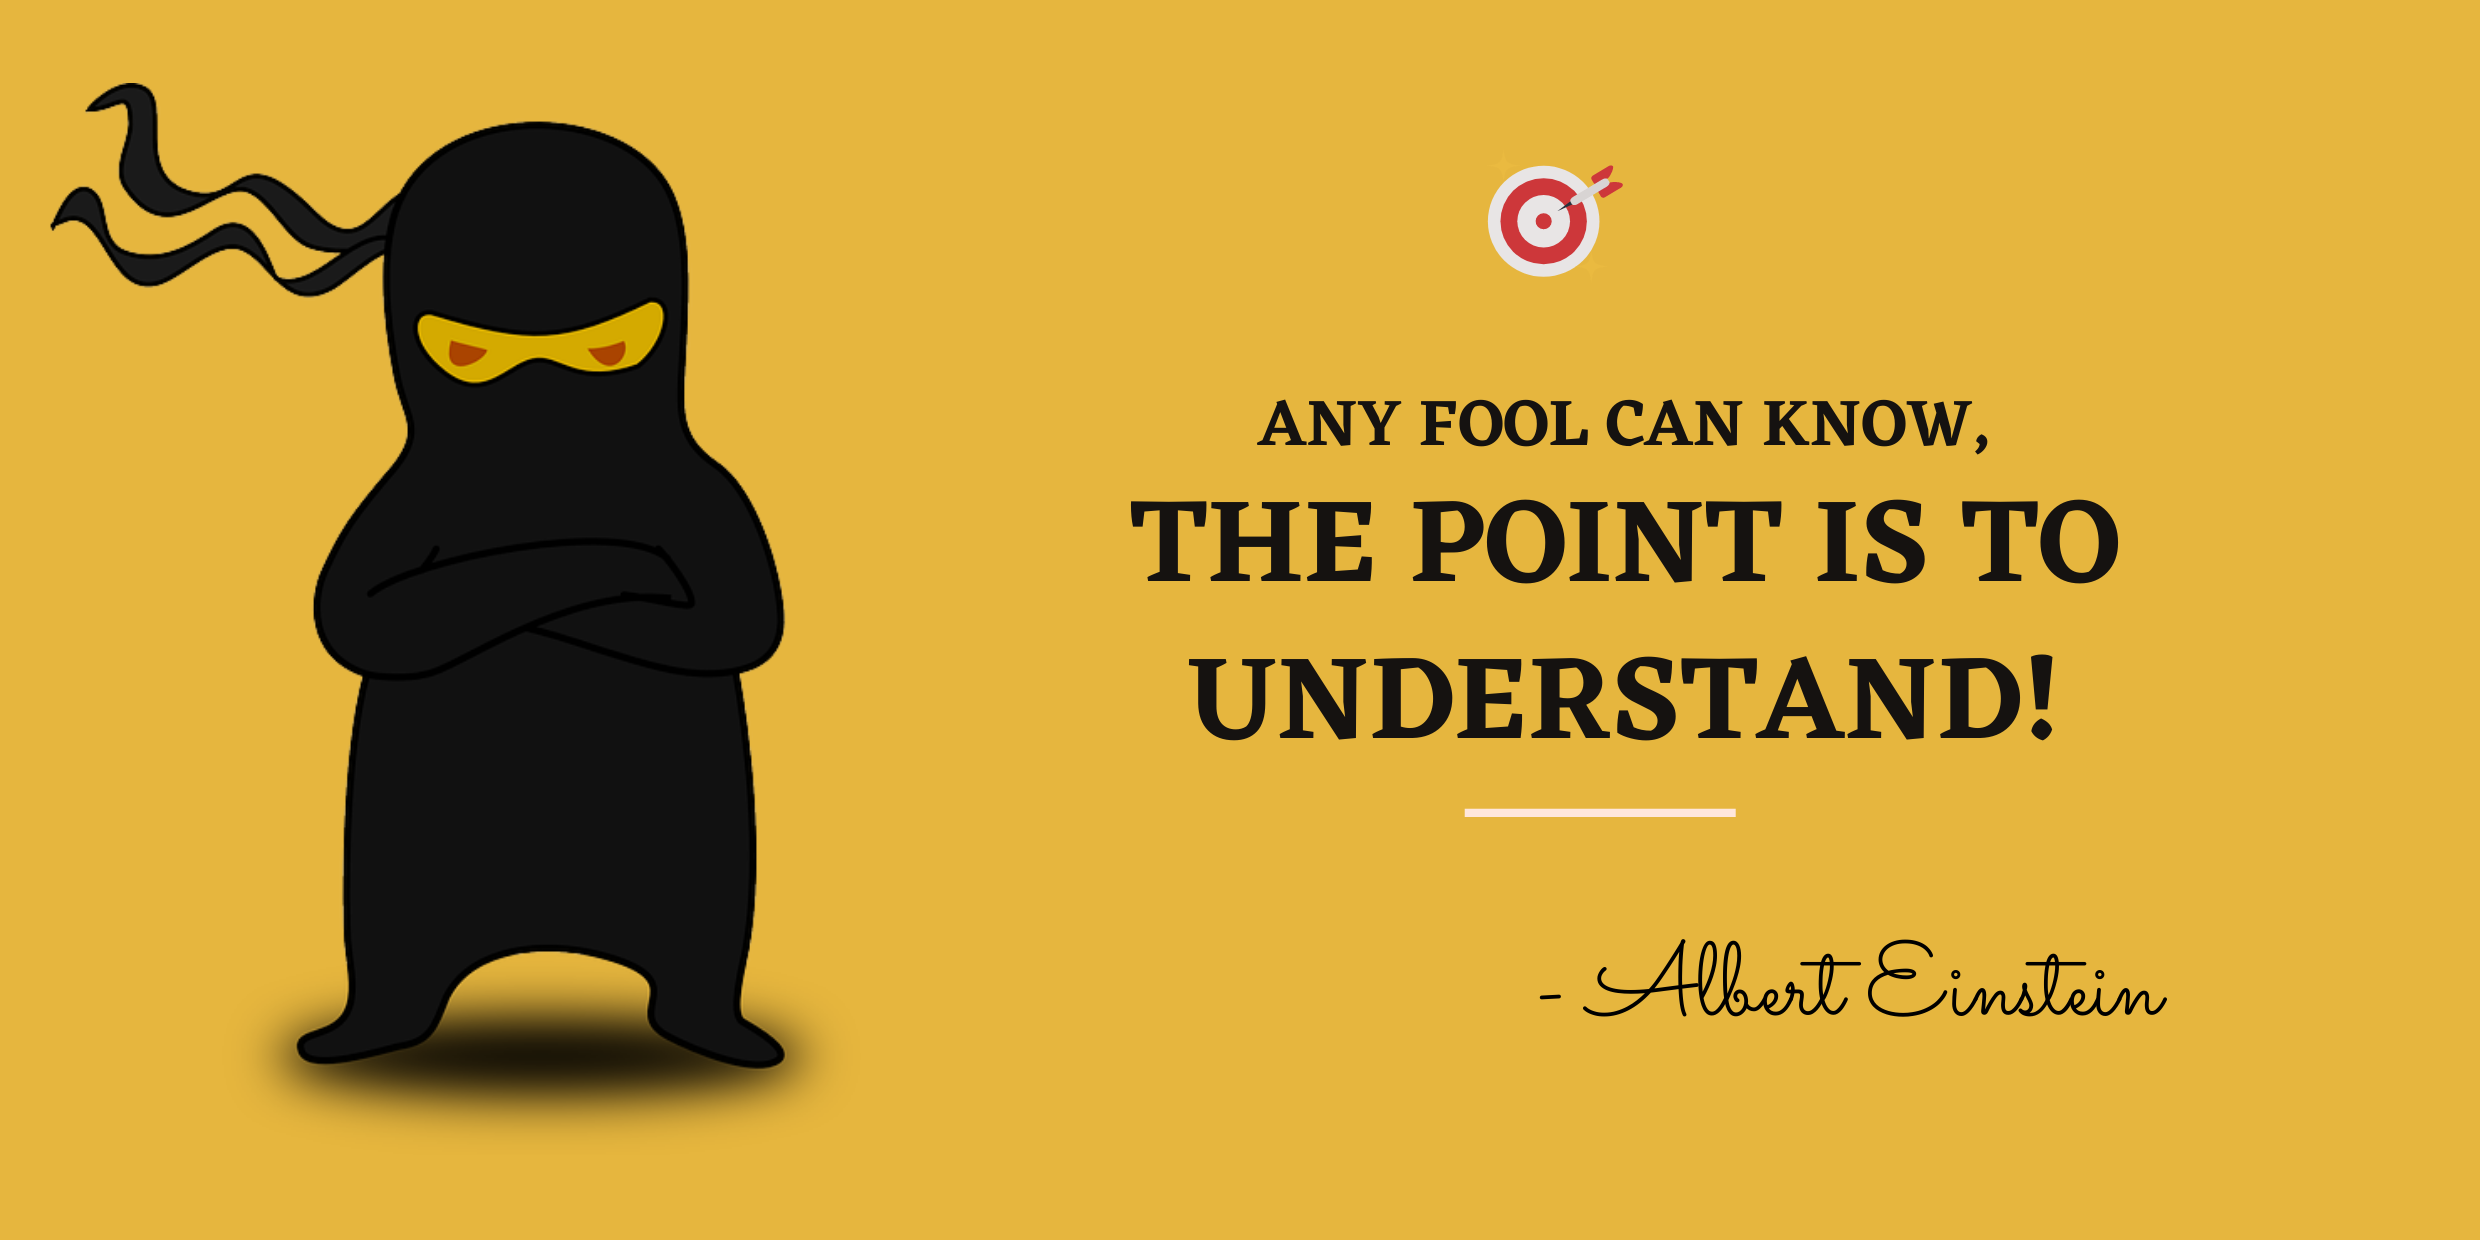
\includegraphics[scale=.2]{content/practise.jpg}
	\end{figure}	
	\begin{enumerate}
		\item \textbf{What is an Operating System? (Select all that applies.)}
		\begin{enumerate}[label=(\alph*)]
			\item A software used for only gaming purpose.
			\item Collection of software that acts as an interface between a user and computer hardware. %correct
			\item OS consists of kernel to interact with hardware, shell and utilities. %correct
			\item OS is a software used for accounting purpose. %correct
			%\item \light{Handling system calls}
		\end{enumerate}
		\bigskip
		\bigskip
		\item \textbf{Which of the following are the functions of a kernel? (Select all that applies.)}
		\begin{enumerate}[label=(\alph*)]
			\item Perform memory management by keeping track of memory. %correct
			\item Perform hardware management. %correct
			\item Establish communication between hardware and software. %correct
			\item Control all processes of the OS. %correct
		\end{enumerate}
		\bigskip
		\bigskip
		\item \textbf{State whether true or false. Kernel is an interface between hardware and software.}
		\begin{enumerate}[label=(\alph*)]
			\item True %correct
			\item False
		\end{enumerate}
	\end{enumerate}
	

\end{flushleft}

\newpage